\documentclass[../poliXuniversity_hospital_(USP)_report.tex]{subfiles}
\graphicspath{ {images/}{../images/}{../../images/} }

\begin{document}

A primeira versão do software do robô hospitalar não era muito convidativa. Ela, por mais que fosse funcional e tivesse inúmeras qualidades, ainda era um código desorganizado, não tinha nenhuma documentação e quase nenhum padrão. De fato, o era evidente que foi um software feito de forma corrida, individualmente e sem nenhuma intenção de deixar fácil de se entender.

Para a segunda versão do robô hospitalar, todo o software do robô foi refeito por completo, porém, dessa vez, tomando muito cuidado com parametrização de códigos, separação de longos scripts e vários arquivos organizados menos com nomes bem intuitivos, documentação de tudo que foi feito, adição de orientação a objetos para construção dos algoritmos e por fim e mais importante, a adição do Git \cite{git21} e GitHub \cite{github21}, junto ao Gitflow, para armazenar os códigos desenvolvidos e conciliar o trabalho em grupo.

Essa formulação foi feita com intuito de tornar o software do robô hospitalar organizado, padronizado e de fácil compreensão para os eventuais membros novos que irão entrar para o projeto do robô hospitalar, dessa forma, podendo dar continuidade ao trabalho sem muitas dificuldades.

Assim como a primeira versão, para a segunda versão foi utilizado o framework ROS (Robotic Operational System) \cite{ROS21} associado ao simulador Gazebo \cite{gazebo21}  para construção de todos os algoritmos de controle de controle do robô hospitalar.
\clearpage

\chapter{Ambiente de Simulação}

Quando falamos em ambiente de simulação emular algum robô de maneira geral, a primeira dúvida que surge é \textbf{“por que simular?”}.

Quando falamos de emular o robô hospitalar, existem dois motivos principais que justificam o esforço de simular um sistema autônomo. O primeiro é a capacidade de pôr o projeto à prova sem a necessidade dos recursos físicos para isso. Tornamos o desenvolvimento de código mais dinâmico, pois não estamos limitados pelo meio físico. Outra vantagem menos óbvia é a garantia de repetibilidade dos testes, ou seja, podemos testar o sistema diversas vezes com as exatas mesmas condições, de modo a entender melhor o comportamento e as respostas do sistema simulado.

Pensando na grande área da engenharia mecânica, é muito mais fácil, rápido e barato simular o comportamento de uma peça no computador do que fabricá-la e aplicar um teste de impacto nela. O processo de projetar uma peça se torna mais eficiente e dinâmico, pois podemos testar diversas configurações e encontrar entre elas qual a mais adequada às nossas necessidades.

Por conta desses dois motivos, foi construído um ambiente de simulação para o robô hospitalar, pois os integrantes do projeto poderiam construir algoritmos de controle e visão computacional sem necessariamente estar com robô físico para realizar os teste, o que era de extrema importância, levando em consideração que toda a segunda versão do projeto foi construído em um período de isolamento social. A sitaução da simulação atualmente pode ser vista nas figuras  ~\ref{Simulação Atualmente - Gazebo} e ~\ref{Simulação Atualmente - Rviz}.

Mesmo assim, vale lembrar que, por mais que a simulação seja convidativa e muito boa, não substitui o teste na realidade. Por melhor que a simulação seja, quem entra no hospital é o robô físico e por melhor que seja a lógica de controle, não existe algoritmo para corrigir parafuso solto ou falta de rigidez na estrutura.

\begin{figure}[h]
\centering
    \caption{Simulação Atualmente - Gazebo}
    \centering % para centralizarmos a figura
    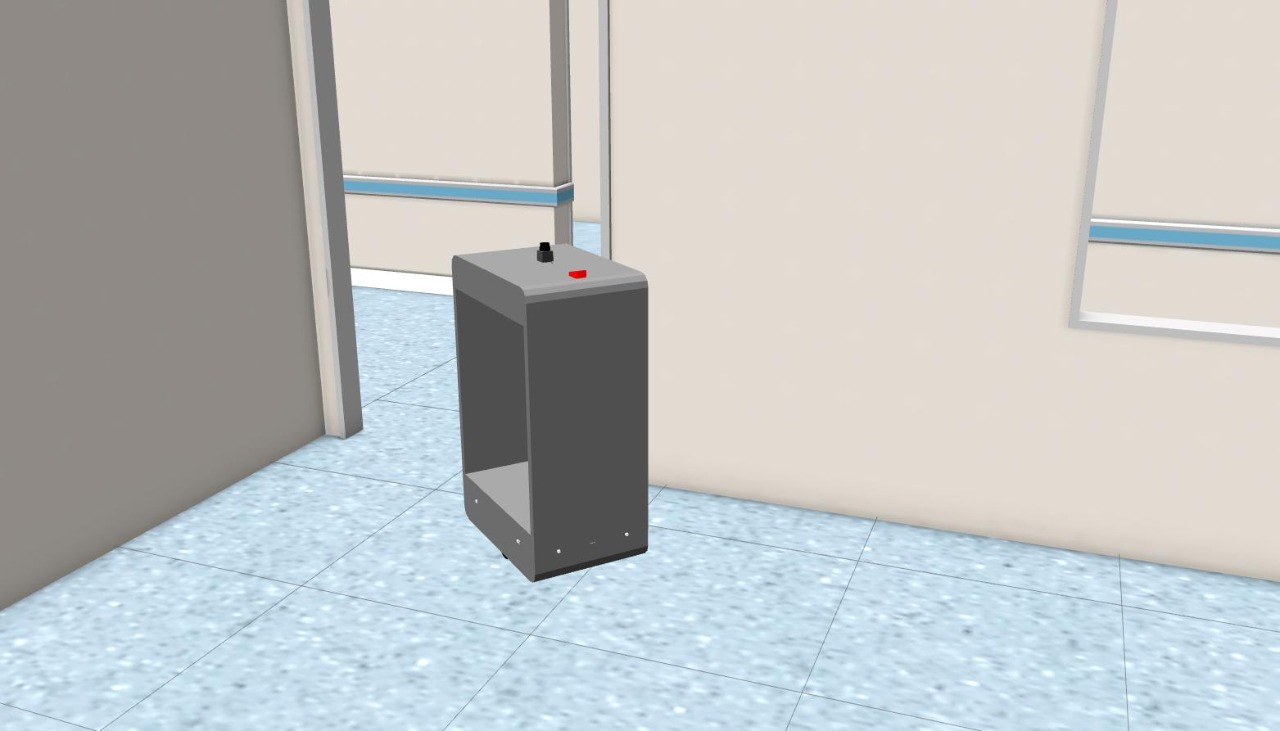
\includegraphics[width=14cm]{simulacao_atual.jpg}
    \caption*{Fonte: Elaborada pelo autor no Software Gazebo \cite{gazebo21}}
    \label{Simulação Atualmente - Gazebo}
\end{figure}

\begin{figure}[h]
\centering
    \caption{Simulação Atualmente - Rviz}
    \centering % para centralizarmos a figura
    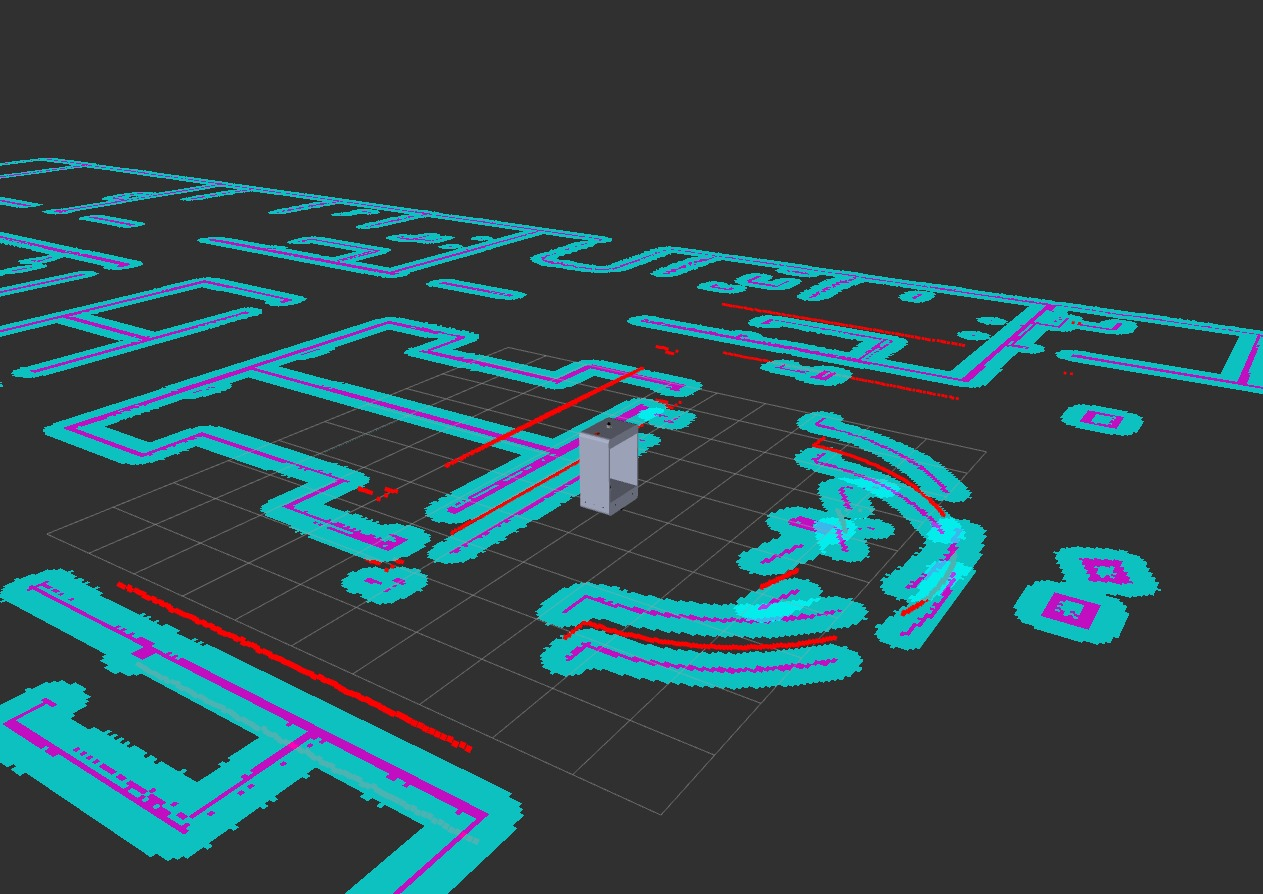
\includegraphics[width=14cm]{simulacao_atual2.jpg}
    \caption*{Fonte: Elaborada pelo autor no Software Rviz\cite{rviz21}}
    \label{Simulação Atualmente - Rviz}
\end{figure}

\clearpage

\section{Gazebo}

%------------------------------------------
\begin{wrapfigure}{r}{5.5cm}
\centering
\caption{Simulador Gazebo}\label{wrap-fig:1}

\includegraphics[width=4cm]{gazebo.png}
\caption*{Fonte: Foto disponibilizada por gazebosim.org}\label{wrap-fig:1}
\end{wrapfigure} 
%------------------------------------------

Dentro do conjunto de pacotes que constituem o ROS \cite{ROS21}, um dos mais famosos no quesito de simulação de robôs autônomos e utilizados é o Gazebo. Nele podemos simular o comportamento dinâmico de um robô, seu movimento e a leitura de seus sensores em diferentes ambientes, cenários e situações programados, de modo a testar todo o algoritmo de controle do robô sem a necessidade ter o robô físico.

Por mais que o Gazebo \cite{gazebo21} faça parte dos pacotes padrões do ROS, ele funciona de forma independente, ou seja, podemos utilizar o simulador sem outro software como requisito.

\section{Modelo do Robô}

Quando falamos em construir um modelo 3D de robô no Gazebo, precisamos descrever sucintamente como ele se comporta mecanicamente, como onde tem junções, e sensorial, como mencionando o como o sensor se comporta e onde se localiza. 

O projeto em CAD do Robô hospitalar foi feito no SolidWorks  \cite{solidworks21} e  Fusion 360 \cite{fusion36021}. Porém o gazebo não suporta arquivos de CAD diretamente na simulação, são suportados 3 tipos de arquivo: .urdf, .xacro e .sdf. Entretanto, tanto o SolidWorks quanto o Fusion têm a opção de exportar os modelos 3D construídos para esses formatos suportados pelo Gazebo, o que facilitou muito o nosso trabalho de criação de um modelo.


Os 3 formatos correspondem a arquivos com estrutura XML. O URDF é o mais simples do 3, o formato xacro é igual ao URDF com a adição ao suporte de macros dentro no arquivo, o que permite fazer a divisão de um código longo em vários pequenos e organizados. Para completar, o formato SDF é mais novo e possui suporte a uma maior quantidade de informações na descrição do modelo do robô, como fator de atrito e amortecimento nas juntas do robô.

Internamente, o Gazebo converte todas as entradas para SDF. Nós utilizamos o formato URDF para o modelo da carenagem porque existe uma extensão de SolidWorks que exporta um arquivo .urdf a partir de um CAD de Assembly.

\subsection{Estrutura XML}

No universo da engenharia de software da robótica, em geral, é muito comum o uso da estrutura XML para descrever as relações entre as diferentes peças e partes de um robô. Um robô descrito em URDF é composto por duas entidades: links e joints

Segundo a documentação oficial do Gazebo \cite{ros_wiki21},as joints são a descrição de como juntamos duas estruturas diferente em um URDF, assim, 
ela meio que descreve os graus de liberdade de determinada junção. O gazebo tem uma série de junções permitidas:

\begin{itemize}
  \item revolute - Revolução ao redor de um eixo com limite de posição, como um servo;
  \item continuous - Revolução ao redor de um eixo sem limite de posição, como um motor DC ou motor de passo;
  \item prismatic - Vínculo deslizante ao longo de um eixo com limite de posição, como um carro em uma guia;
  \item fixed - Vínculo de travamento, no qual os 6 graus de liberdade estão fixos. Descreve o vínculo entre duas peças que não possuem movimento relativo;
  \item floating - Vínculo sem restrição em nenhum dos 6 graus de liberdade;
  \item planar - Vínculo de movimento em um plano perpendicular a um eixo especificado.
\end{itemize}

Os links estão organizados em uma estrutura de dados de árvore, na qual links país (como o corpo) se conectam com links filhos (como as roda ou sensor) por meio de joints, que descrevem o vínculo existente entre os links. Essa estrutura serve para relacionar os diferentes sistemas de coordenadas dos vários links, como pode ser visto na figura \ref{fig:Estrutura URDF - Visão Greal} e \ref{fig:Estrutura URDF - Visão Física}

\begin{figure}[!h]
    \centering
    \begin{minipage}{0.5\textwidth}
        \centering
        \caption{Estrutura URDF - Visão Física}
        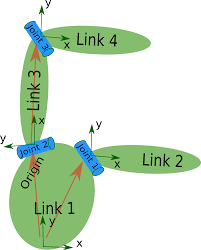
\includegraphics[width=0.68\textwidth]{urdf_idea.png} 
        \label{fig:Estrutura URDF - Visão Física}
    \end{minipage}\hfill
    \begin{minipage}{0.5\textwidth}
        \centering
        \caption{Estrutura URDF - Visão Geral}
        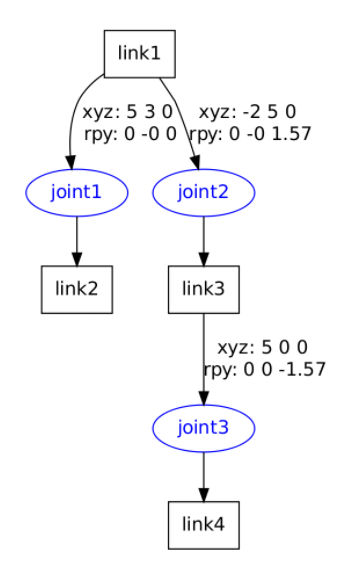
\includegraphics[width=0.5\textwidth]{urdf_idea2.png} 
        \label{fig:Estrutura URDF - Visão Greal}
    \end{minipage}\hfill
    
    \caption*{Fonte: retidado do site <http://library.isr.ist.utl.pt/> }
    \label{fig:Protótipo Sinalização - PCB 2D3D}
\end{figure}

\subsection{Carenagem}

O CAD completo da carenagem do robô era muito complexo. Havia um número muito grande de parafusos e outros detalhes mecânicos que tornaria a simulação muito custosa sem um bom custo benefício. Por conta disso foi elaborado um modelo simplificado da estrutura principal do robô.

Além disso, uma simulação muitos custosa deixaria inviável a utilização da mesma nos computadores domésticos que a maioria dos membros do projeto tem. Por conta disso, deixar a simulação mais eficiente era necessário para todo mundo dar continuidade ao trabalho a distância.

Nessa estrutura principal, se deu prioridade principalmente ao formato geral do robô, peso e momento de inércia e principalmente na construção sensorial do robô. Dessa forma, podendo realizar um ótima simulação e não ter um custo computacional muito elevado. 

\begin{figure}[h]
\centering
    \caption{Modelo Simulado da Robô Hospitalar (V2)}
    \centering % para centralizarmos a figura
    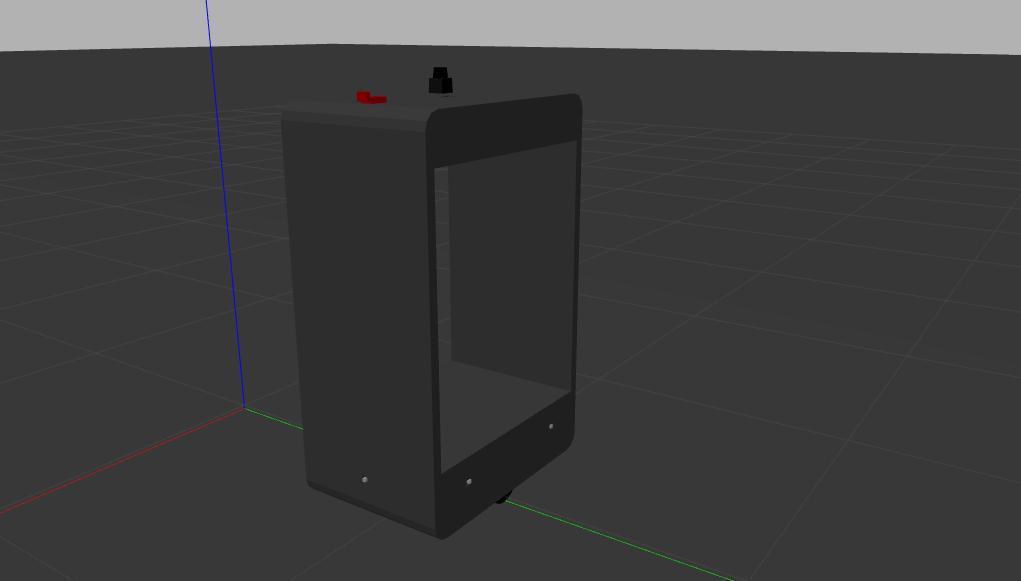
\includegraphics[width=14cm]{modelo_robo_hospitalar.jpg}
    \caption*{Fonte: Elaborada pelo autor no Software Gazebo\cite{gazebo21}}
    \label{figura:1° Versão Robô Hospitalar}
\end{figure}
 
\clearpage 
\subsubsection{Estrutura do URDF - Carenagem}
\begin{lstlisting}
root Link: base has 14 child(ren)
    child(1):  left_back_back_castor_mount_link
        child(1):  left_back_castor_dummy_link
            child(1):  left_back_castor_wheel_link
    child(2):  left_front_castor_mount_link
        child(1):  left_front_castor_dummy_link
            child(1):  left_front_castor_wheel_link
    child(3):  right_back_castor_mount_link
        child(1):  right_back_castor_dummy_link
            child(1):  right_back_castor_wheel_link
    child(4):  right_front_castor_mount_link
        child(1):  right_front_castor_dummy_link
            child(1):  right_front_castor_wheel_link
    child(5):  camera_link
    child(6):  link_back_left_proximity
    child(7):  link_back_proximity
    child(8):  link_back_right_proximity
    child(9):  link_front_left_proximity
    child(10):  link_front_proximity
\end{lstlisting}

\subsection{Sensores}

Depois de importar corretamente o modelo 3D, é necessário adicionar a descrição funcional e física do sensor no seu modelo de sensor. 

Para realizar descrição, é necessário adicionar um \texttt{ plugin} no Gazebo, que consiste em criar um arquivo que contém toda a descrição física, lógica e conexão(relacionado com as joints).

No caso do robô hospitalar, era necessário adicionar sensores de distância, lidar, câmera e encoder. Para cada um desses sensores, com exceção do encoder, que ainda não foi implementado, todos os outros receberam um um arquivo individual no repositório individual da simulação.

O modelo do robô com os sensores funcionando pode ser visto na figura \ref{fig:Sensores Simulado da Robô Hospitalar (V2)}

\begin{figure}[h]
\centering
    \caption{Sensores Simulado da Robô Hospitalar (V2)}
    \centering % para centralizarmos a figura
    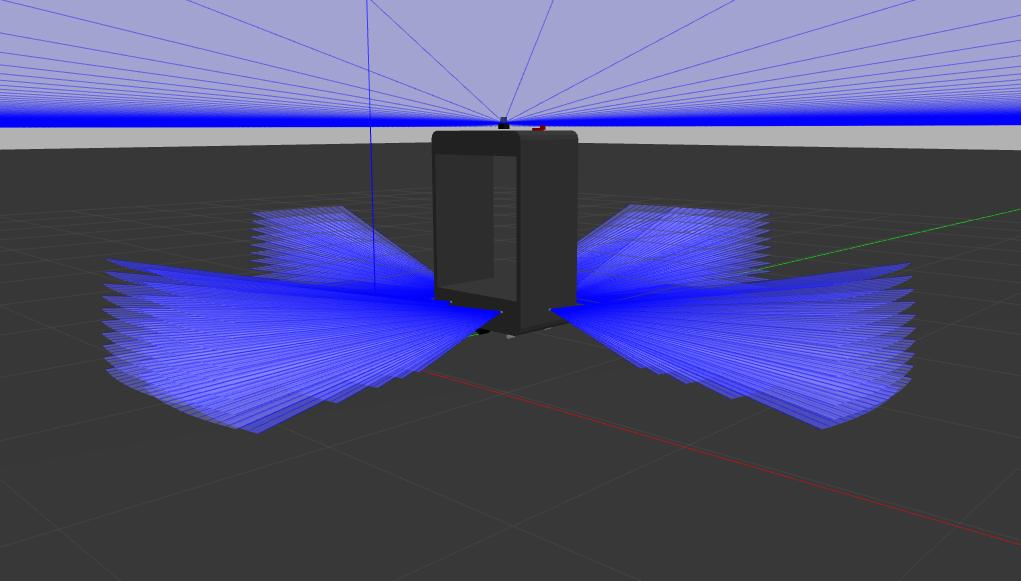
\includegraphics[width=14cm]{modelo_robo_sensores.jpg}
    \caption*{Fonte: Elaborada pelo autor no Software Gazebo\cite{gazebo21}}
    \label{fig:Sensores Simulado da Robô Hospitalar (V2)}
\end{figure}

\subsubsection{Rviz}


\begin{figure}[h]
\centering
    \caption{Sensores Simulado no Rviz da Robô Hospitalar (V2)}
    \centering % para centralizarmos a figura
    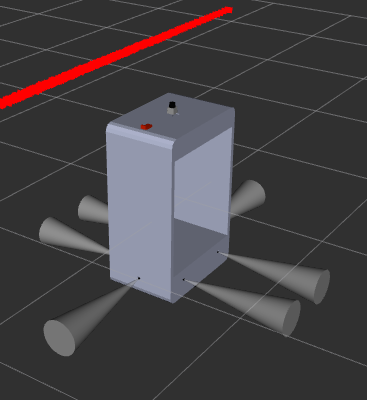
\includegraphics[width=10cm]{robo_rviz.png}
    \caption*{Fonte: Elaborada pelo autor no Software Rviz\cite{rviz21}}
    \label{fig:Sensores Simulado no Rviz da Robô Hospitalar (V2)}
\end{figure}

Para visualizar os dados coletados pelo robô e como processa essa informação, principalmente associada aos tópicos publicados, usamos outro framework associado ao ROS, o Rviz.

Com o auxílio do Rviz, podemos entender melhor como os dados obtidos pelos sensores do robô estão sendo processados e traduzidos para o ponto de vista do robô. Na figura ~\ref{fig:Sensores Simulado no Rviz da Robô Hospitalar (V2)}, pode-se ver o  modelo do robô hospitalar no Rviz. Na parte inferior, é exposto como os dados do sensor de distância estão sendo vistos pelo robô e na parte superior, a parte em vermelho, é como os dados do lidar estão sendo vistos.


\section{Modelo do mundo}

Para uma boa simulação, não basta somente termos o modelo físico do robô bem estruturado, precisamos adicionar o nosso robô em um ambiente que ele realmente estará imerso na vida real. Para isso, é necessário criar um mundo (vindo do termo  \texttt{world}) no caso para adicionarmos o nosso robô.

Por se tratar de um robô hospitalar,  o melhor ambiente possível para deixar o robô imerso em um hospital ou algo similar a isso. Entretanto, criar um mundo do zero no gazebo é uma experiência muito demorada e minuciosa, por conta disso, o grupo optou por usar um mapa de hospital já pronto e disponibilizado pela Amazon para uso no AWS no GitHub, tal repositório pode ser visto aqui \cite{hospital_world21}.

Com o mapa disponibilizado pela Amazon, que disponibiliza um ambiente ideal para simulação do robô hospitalar, podemos por fim completar todo o ambiente de simulação e começar a desenvolver os algoritmos básicos de controle do robô hospitalar.



\begin{figure}[h]
\centering
    \caption{AWS RoboMaker Hospital World - vista pela frente}
    \centering % para centralizarmos a figura
    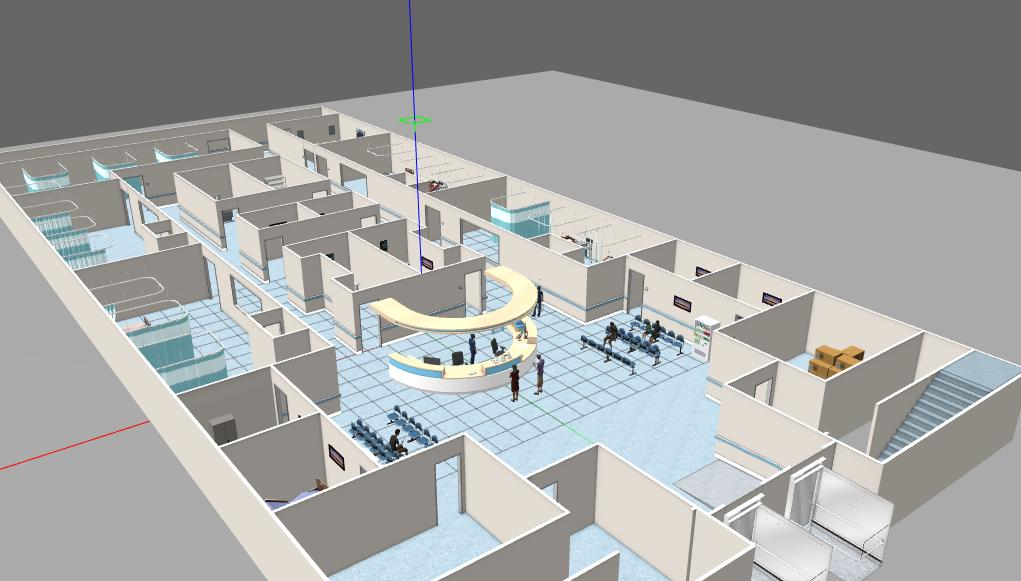
\includegraphics[width=15cm]{d_hworld1.jpg}
    \caption*{Fonte: Elaborada pelo autor no Software Gazebo\cite{gazebo21}}
    \label{fig:AWS RoboMaker Hospital World - vista pela frente}
\end{figure}

\begin{figure}[h]
\centering
    \caption{AWS RoboMaker Hospital World - vista por trás}
    \centering % para centralizarmos a figura
    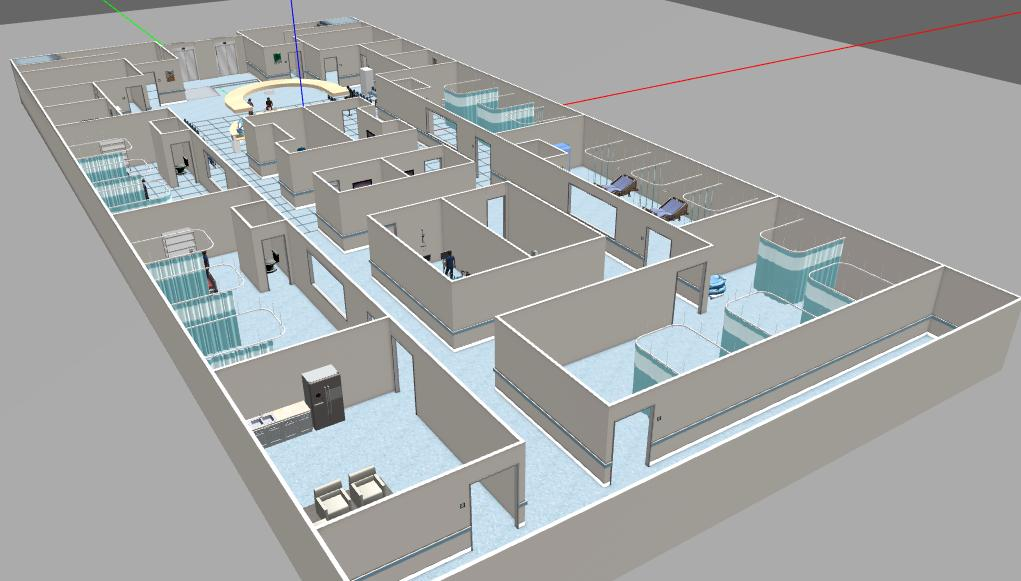
\includegraphics[width=15cm]{d_hworld2.jpg}
    \caption*{Fonte: Elaborada pelo autor no Software Gazebo\cite{gazebo21}}
    \label{fig:AWS RoboMaker Hospital World - vista por trás}
\end{figure}


\begin{comment}
\section{Repositório}
\end{comment}

\end{document}